% \cleardoublepage
\chapter{Summary and Further Work}\minitoc\label{sec:summary}\vspace{.5cm}

\section{Overview}

\begin{wrapfigure}{r}{0.2\textwidth}
    \centering
    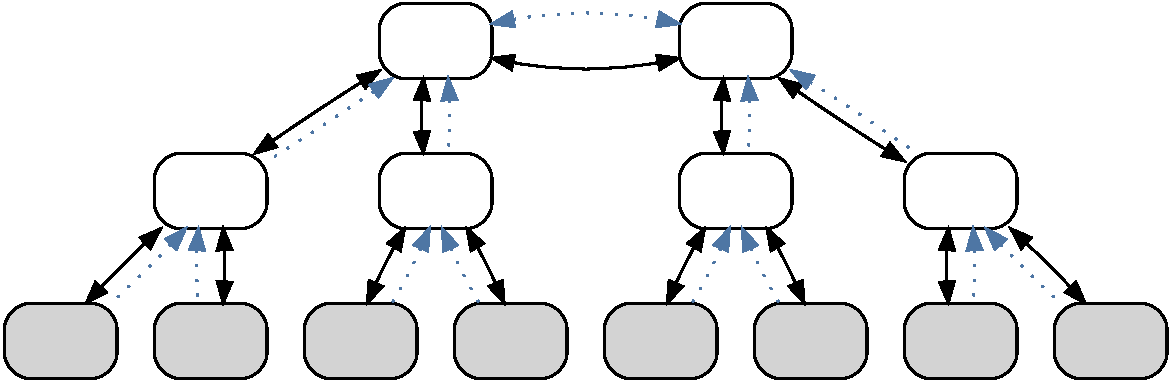
\includegraphics[width=0.2\textwidth]{resources/images/example3}
\end{wrapfigure}

\sidenote{Contributions}
\todomid{write}

\begin{figure}
    \centering
    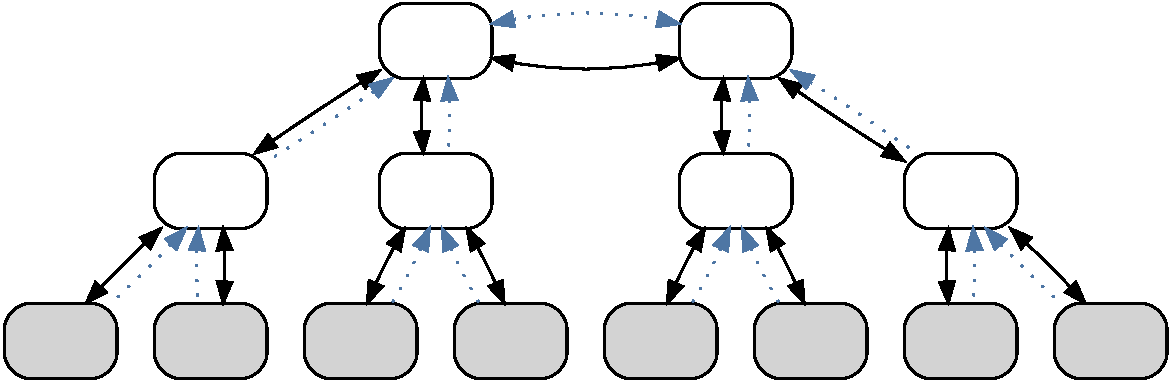
\includegraphics[width=.55\textwidth]{resources/images/example3}
    \caption{Placement of the outlook in the structure of research}\label{fig:hourglass:outlook}
\end{figure}

\sidenote{Dissemination}
\todomid{write about \Cref{fig:hourglass:outlook}}

\section{Conclusions and Impact}

\sidenote{Context}
\todomid{write}

\sidenote{Contribution 1}
\todomid{write}

\sidenote{Contribution 2}
\todomid{write}

\sidenote{Contribution 3}
\todomid{write}

\section{Outlook}

\sidenote{Intro}
\todomid{write}

\sidenote{Application Area 1}
\todomid{write about \Cref{fig:outlook:aa1}}

\begin{figure}
    \centering
    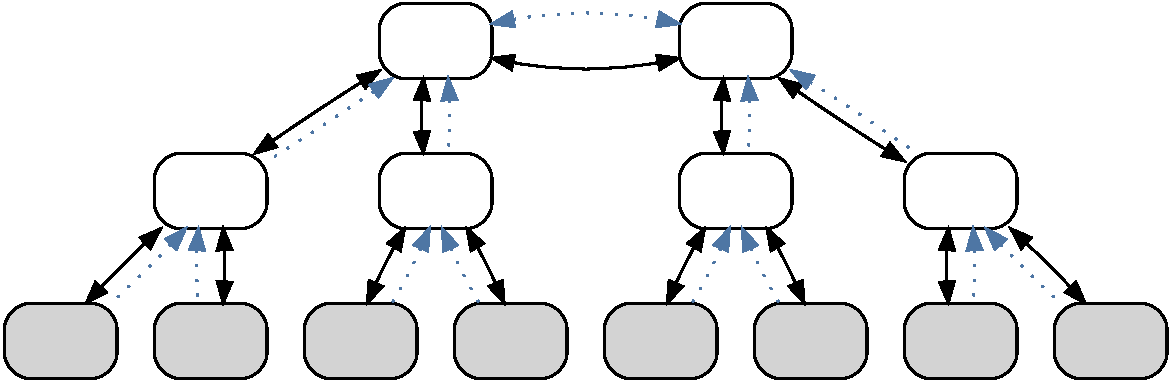
\includegraphics[width=.85\textwidth]{resources/images/example3}
    \caption{Area 1~\cite{li2002design}}\label{fig:outlook:aa1}
\end{figure}

\sidenote{Application Area 2}
\todomid{write}

\sidenote{Application Area 3}
\todomid{write}

\sidenote{Application Area 4}
\todomid{write}
